\documentclass[paper=a4]{article}
\usepackage{ucs}
\usepackage[utf8x]{inputenc}
\usepackage[T1]{fontenc}
\PreloadUnicodePage{0}
\usepackage{xspace}
\usepackage{array}
\usepackage[hmargin=3.5cm,vmargin=2.7cm]{geometry} 
\usepackage{graphicx}



\begin{document}
\title{ \normalsize 
\includegraphics[scale=0.43]{images/CarGameLogo.png}
	\\
	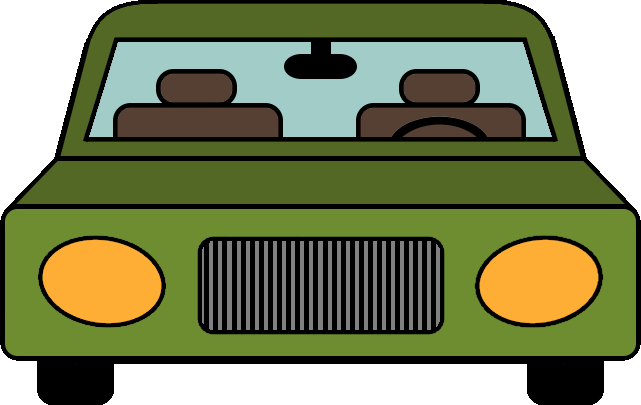
\includegraphics[scale=0.5]{images/menu_car.png}
}
\author{Team Dank \\
Universitetet i Bergern \\
Informatikk}
\maketitle
\newpage

\section{Innholdsliste}
\begin{itemize}
	\item Introduksjon ........................................................................................................... 3
	\item Systemkrav og installasjon ..................................................................................... 4
	\item Spillinstruksjoner og -regler .................................................................................... 5
		\begin{itemize} 
			\item Kontroller
			\item Objekt-interaksjon
			\item Poeng
			\item Penger
			\item Vær
		\end{itemize}
	\item Bilder ....................................................................................................................... noe
	\item Kredit ...................................................................................................................... noe
\end{itemize}
\newpage

\section{Introduksjon}
Som Carl liker du å kjøre uforsvarlig, og målet ditt er å komme deg så lengst mulig uten gå tom for bensin og få mest mulig poeng. \\

Dette er et spill tiltenkt datamaskiner der spilleren kjører en bil.
Bilen kjører langs en vei med forskjellige ting i veibanen, som spilleren kan kjøre over eller unngå.
Vanndammer vil gjøre at spilleren mister drivstoff, og mister litt kontrollen over bilen.
Kumlokk i veien gjør at spilleren taper.
Bensintanker gir spilleren ekstra drivstoff, slik at runden varer lenger.
Myke trafikanter vil gi poeng til spilleren dersom de blir påkjørt.
Mynter kan plukkes opp slik at spilleren kan kjøpe nye biler.
Spilleren får en score for hver spillrunde, i tillegg til at spilleren samler opp virtuelle penger som kan brukes til å bytte bil.
\newpage

\section{Systemkrav og installasjon}
\subsection{Systemkrav}
\begin{itemize}
	\item Ikke mindre enn 1 GB RAM minne\\
	\item Windows Vista/Linux 2005/Mac OS X eller senere \\
	\item 50 MB ledig plass for installasjon \\
	\item Java 8 \\
	\item Tastatur, mus \\
 	\item TeamDank anbefaler deg å ha en prosessor (2005+) med \\ 
klokkefrekvens på 1.6 Ghz eller bedre.
\end{itemize}
\subsection{Installasjon}
Du må først sørge for at du har installert den nyeste versjonen av Java og \\
for å kunne spille Carl the Crasher må du laste ned carlthecrasher.jar-filen. \\
Deretter åpner du filen som vanlig for å starte spillet.   
\newpage

\section{Spillinstruksjoner og -regler} 
\subsection{Kontroll} 
Din primære spillinngangsenhet er tastaturet, og kan gjøre følgende: 
\begin{itemize}
	\item Du styrer Carl til høyre og venstre ved å bruke enten piltastene eller tastaturknappene \\ A og D. 
	\item Carl kan ikke styre bilens hastighet direkte, men farten vil øke jo lenger du kjøre.
	\item Du kan ikke kjøre ut av veien, men du kan kjøre på objekter som oppstår på veien.
	\item Du kan pause spillet ved å gå til pausemenyen ved å trykke på tastaturknappen ESC. 
	\begin{itemize}
		\item Å trykke på ESC vil gi deg muligheten til å fortsette eller avslutte spillet.
	\end{itemize}
\end{itemize}

\subsection{Object-interaksjon}
På veien kan det oppstå forskjellige objekter, og avhengig av objektet kan det påføre bilen en positiv eller negativ effekt. \\
{\renewcommand\labelitemi{}
\begin{itemize}
	\item 
\includegraphics[scale=0.2]{images/gastank.png} \textbf{Bensintank}: Kan plukkes opp for å øke drivstoffet slik at du kan kjøre lengre 
	\item 
\includegraphics[scale=0.5]{images/coin.png} \textbf{Mynt}: På veien kan du finne mynter som du kan plukke opp.
																Myntene kan brukes i butikken for å kjøpe nye biler.
	\item 
\includegraphics[scale=0.2]{images/puddle.png} \textbf{Vanndam}: Kjører du på en vanndam vil det minske mengden drivstoff du har,
																og samtidig gjøre at du vil miste litt kontrollen på bilen i en liten periode. 
	\item 
\includegraphics[scale=0.2]{images/manhole.png} \textbf{Kumlokk}: Dersom du kjører på et kumlokk vil du kræsje og deretter tape umiddelbart.
	\item 
\includegraphics[scale=0.4]{images/walker.png} \textbf{Myke trafikanter}: Å kjøre på trafikanter vil gi deg ekstra poeng som vil øke sluttpoengsummen din.
\end{itemize}
}

\subsection{Poeng}
Målet ditt er å få den høyeste poengsummen, og det finnes ulike måter å tjene opp poeng på:
\begin{itemize}
	\item Du starter alltid med 0 poeng i starten av en runde, \\men du tjener opp poeng konstant når du kjører.
	\item Poeng blir opptjent avhengig av hvor langt du kjører. 
	\item Å kjøre på myke trafikanter vil gi deg poeng, og ulike trafikanter vil gi ulik poengsum.
\end{itemize}

\subsection{Penger} 
\begin{itemize}
	\item{I løpet av spillet får spilleren penger i form av spillets egen valuta.}
	\item{Pengene kan brukes i spillets butikk fra hovedmenyen for å kjøpe nye biler.}
\end{itemize}

\subsection{Vær} 
Spillet vil tilpasse seg etter det lokale værforholdet hos deg. Om det er skyer vil det være skyer på banen,
om det regner vil det regne på banen, og om det snør vil det være snø på banen. \\
Disse dataene om værforholdene blir hentet ut fra yr.no. 
\begin{itemize} 
	\item \textbf{Sol}: Normal framgang.
	\item \textbf{Skyer}: Skyer i spillet, men værforholdet endrer ikke spillets framgang.
	\item \textbf{Regn}: Det regner i spillet og det vil dukke opp flere vanndammer	, samt flere og nye trafikanter. 
	\item \textbf{Snø}: Det er snø på bygningene og andre trafikanter vil dukke opp. Det vil også være vanskeligere å styre bilen,
 og du vil miste mye av kontrollen på bilen dersom du kjører i en vanndam.
\end{itemize}


INSERT PICTURES OF DIFFERENT WEATHERS
\newpage
\section{Bilder}
	\begin{center}
	{\renewcommand\labelitemi{}
		\begin{itemize}
			\item{\makebox[13.5cm]{
\includegraphics[width=1.00\textwidth]{images/main_menu.PNG}}}
			\item {\hfil Figure 1. Hovedmeny} 
			\bigskip
			\bigskip
			\bigskip
			\item{\makebox[13.5cm]{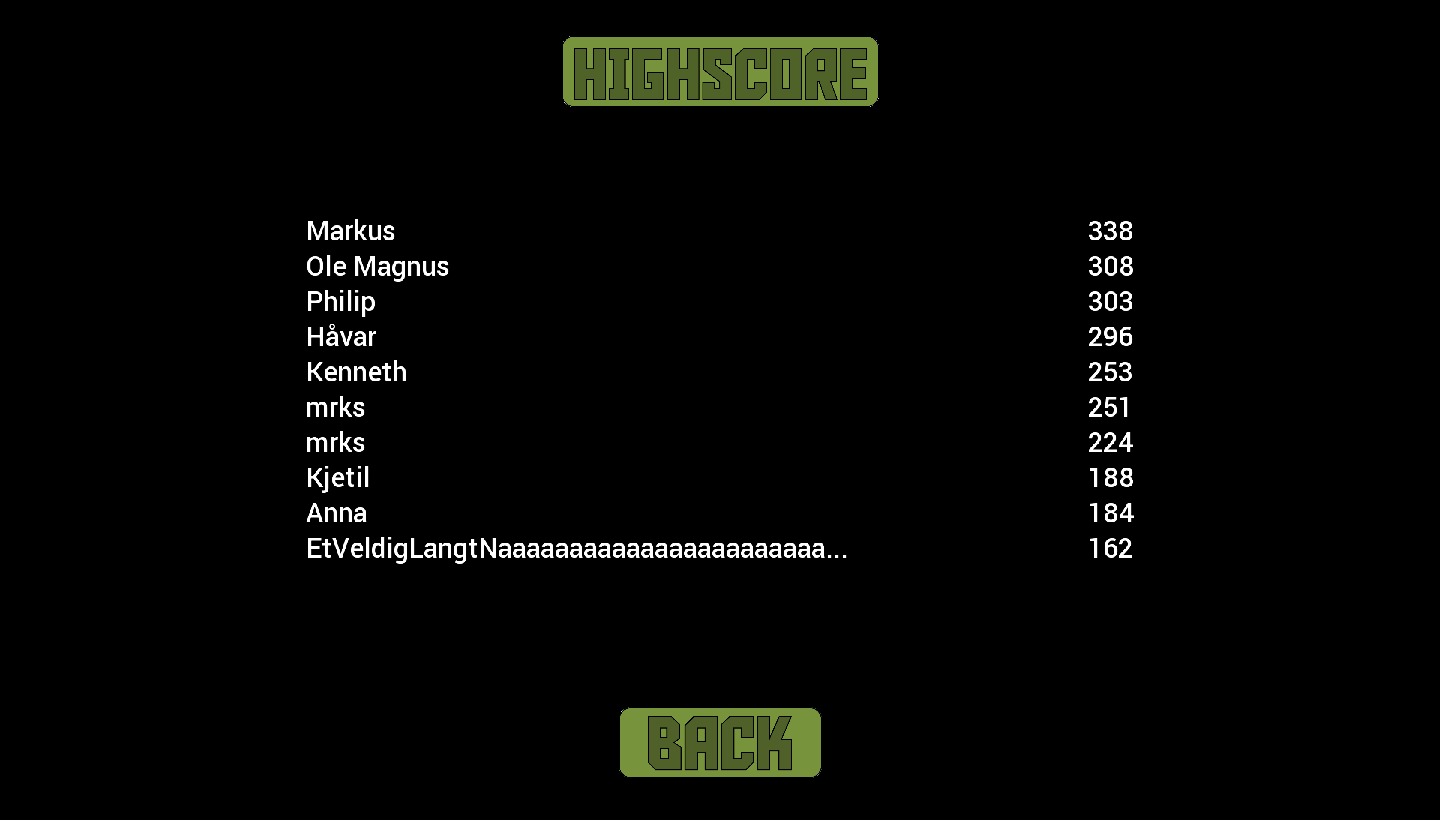
\includegraphics[width=1.00\textwidth]{images/hs_menu.PNG}}}
			\item {\hfil Figure 2. Highscoremeny}
			\bigskip
			\bigskip
			\bigskip
			\item{\makebox[13.5cm]{ 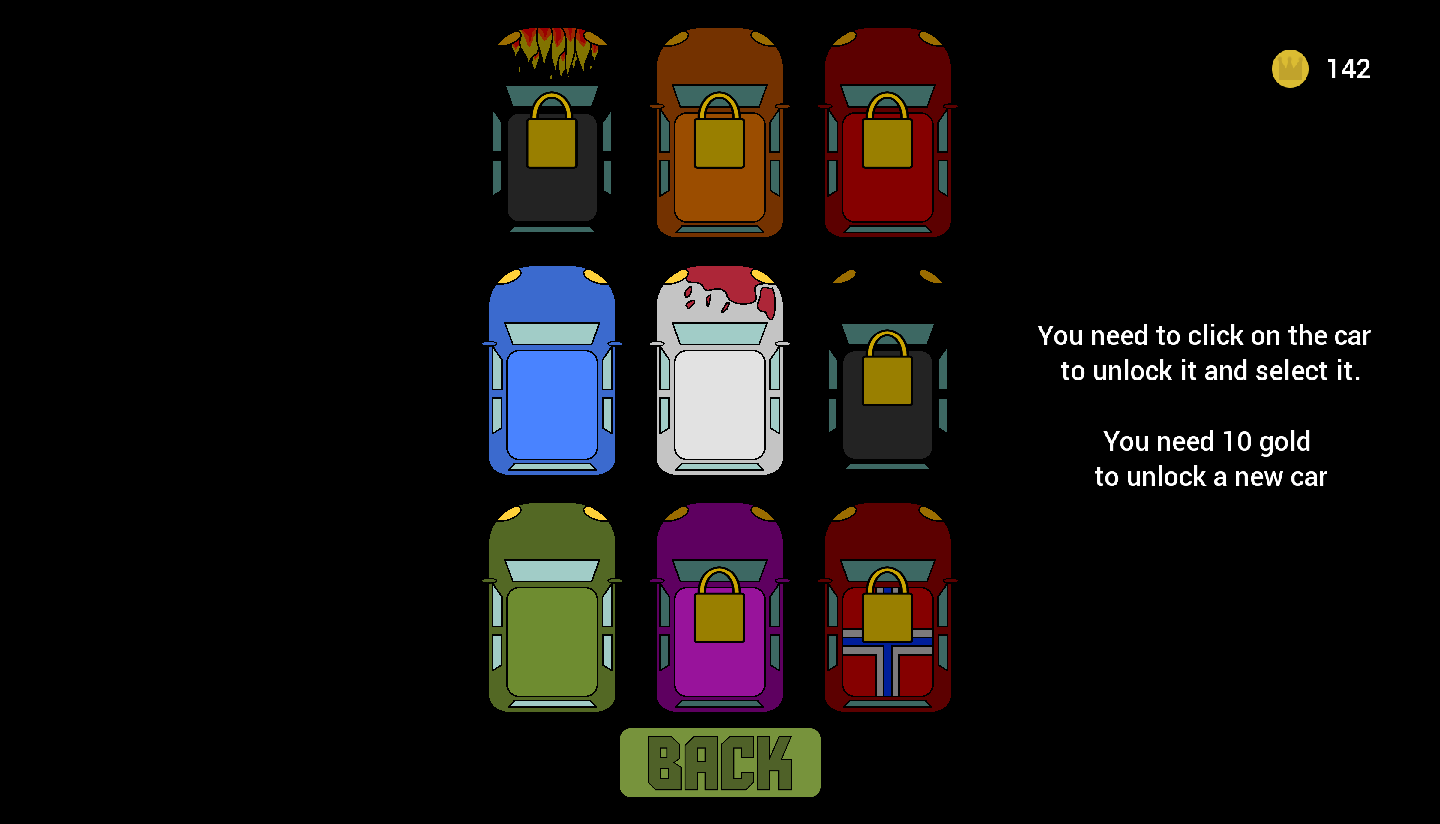
\includegraphics[width=1.00\textwidth]{images/shop_menu.PNG}}}
			\item {\hfil Figure 3. Butikkmeny}
			\bigskip
			\bigskip
			\bigskip
			\item{\makebox[13.5cm]{ 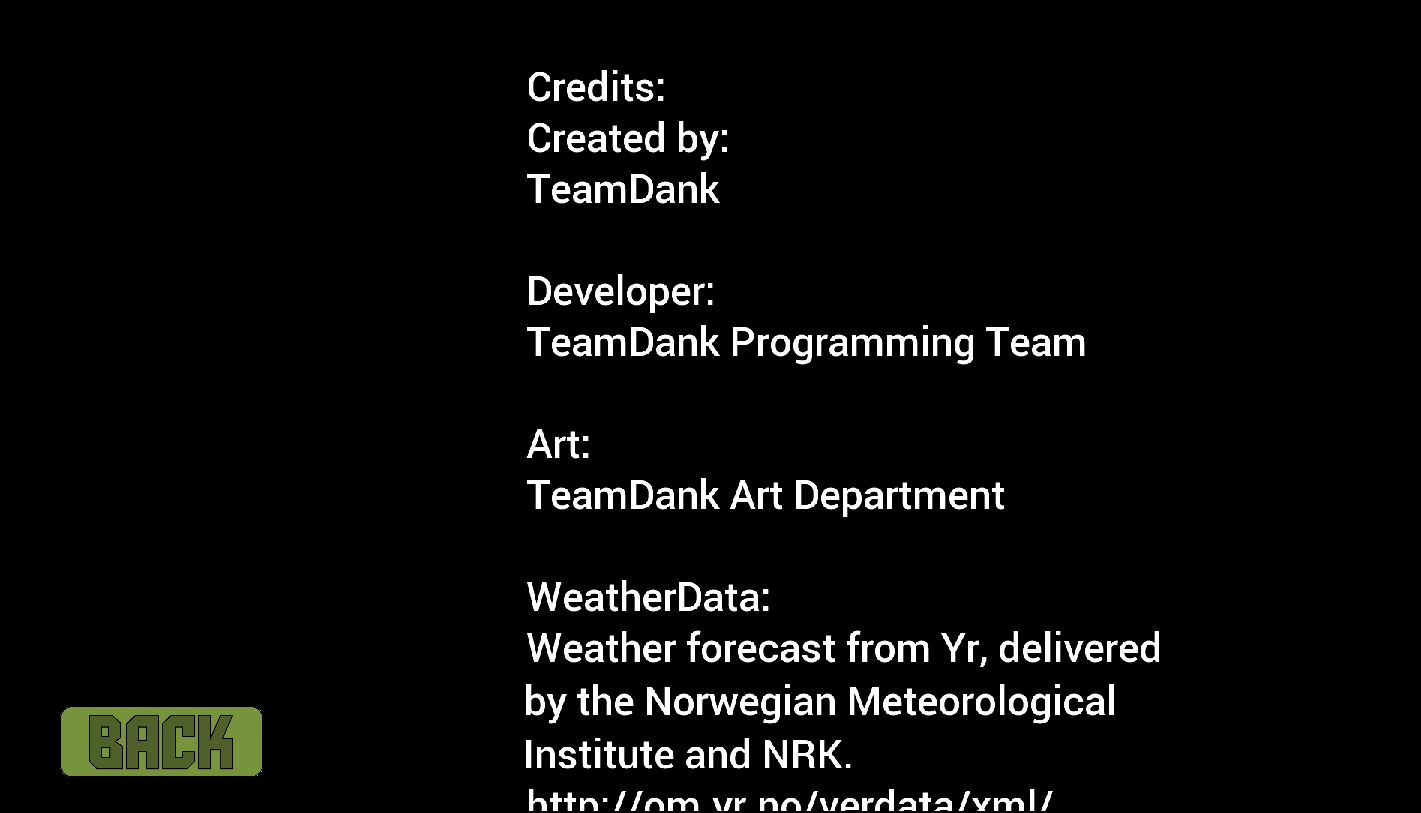
\includegraphics[width=1.00\textwidth]{images/credits.PNG}}}
			\item {\hfil Figure 4. Kreditering}
			\bigskip
			\bigskip
			\bigskip
			\item{\makebox[13.5cm]{ 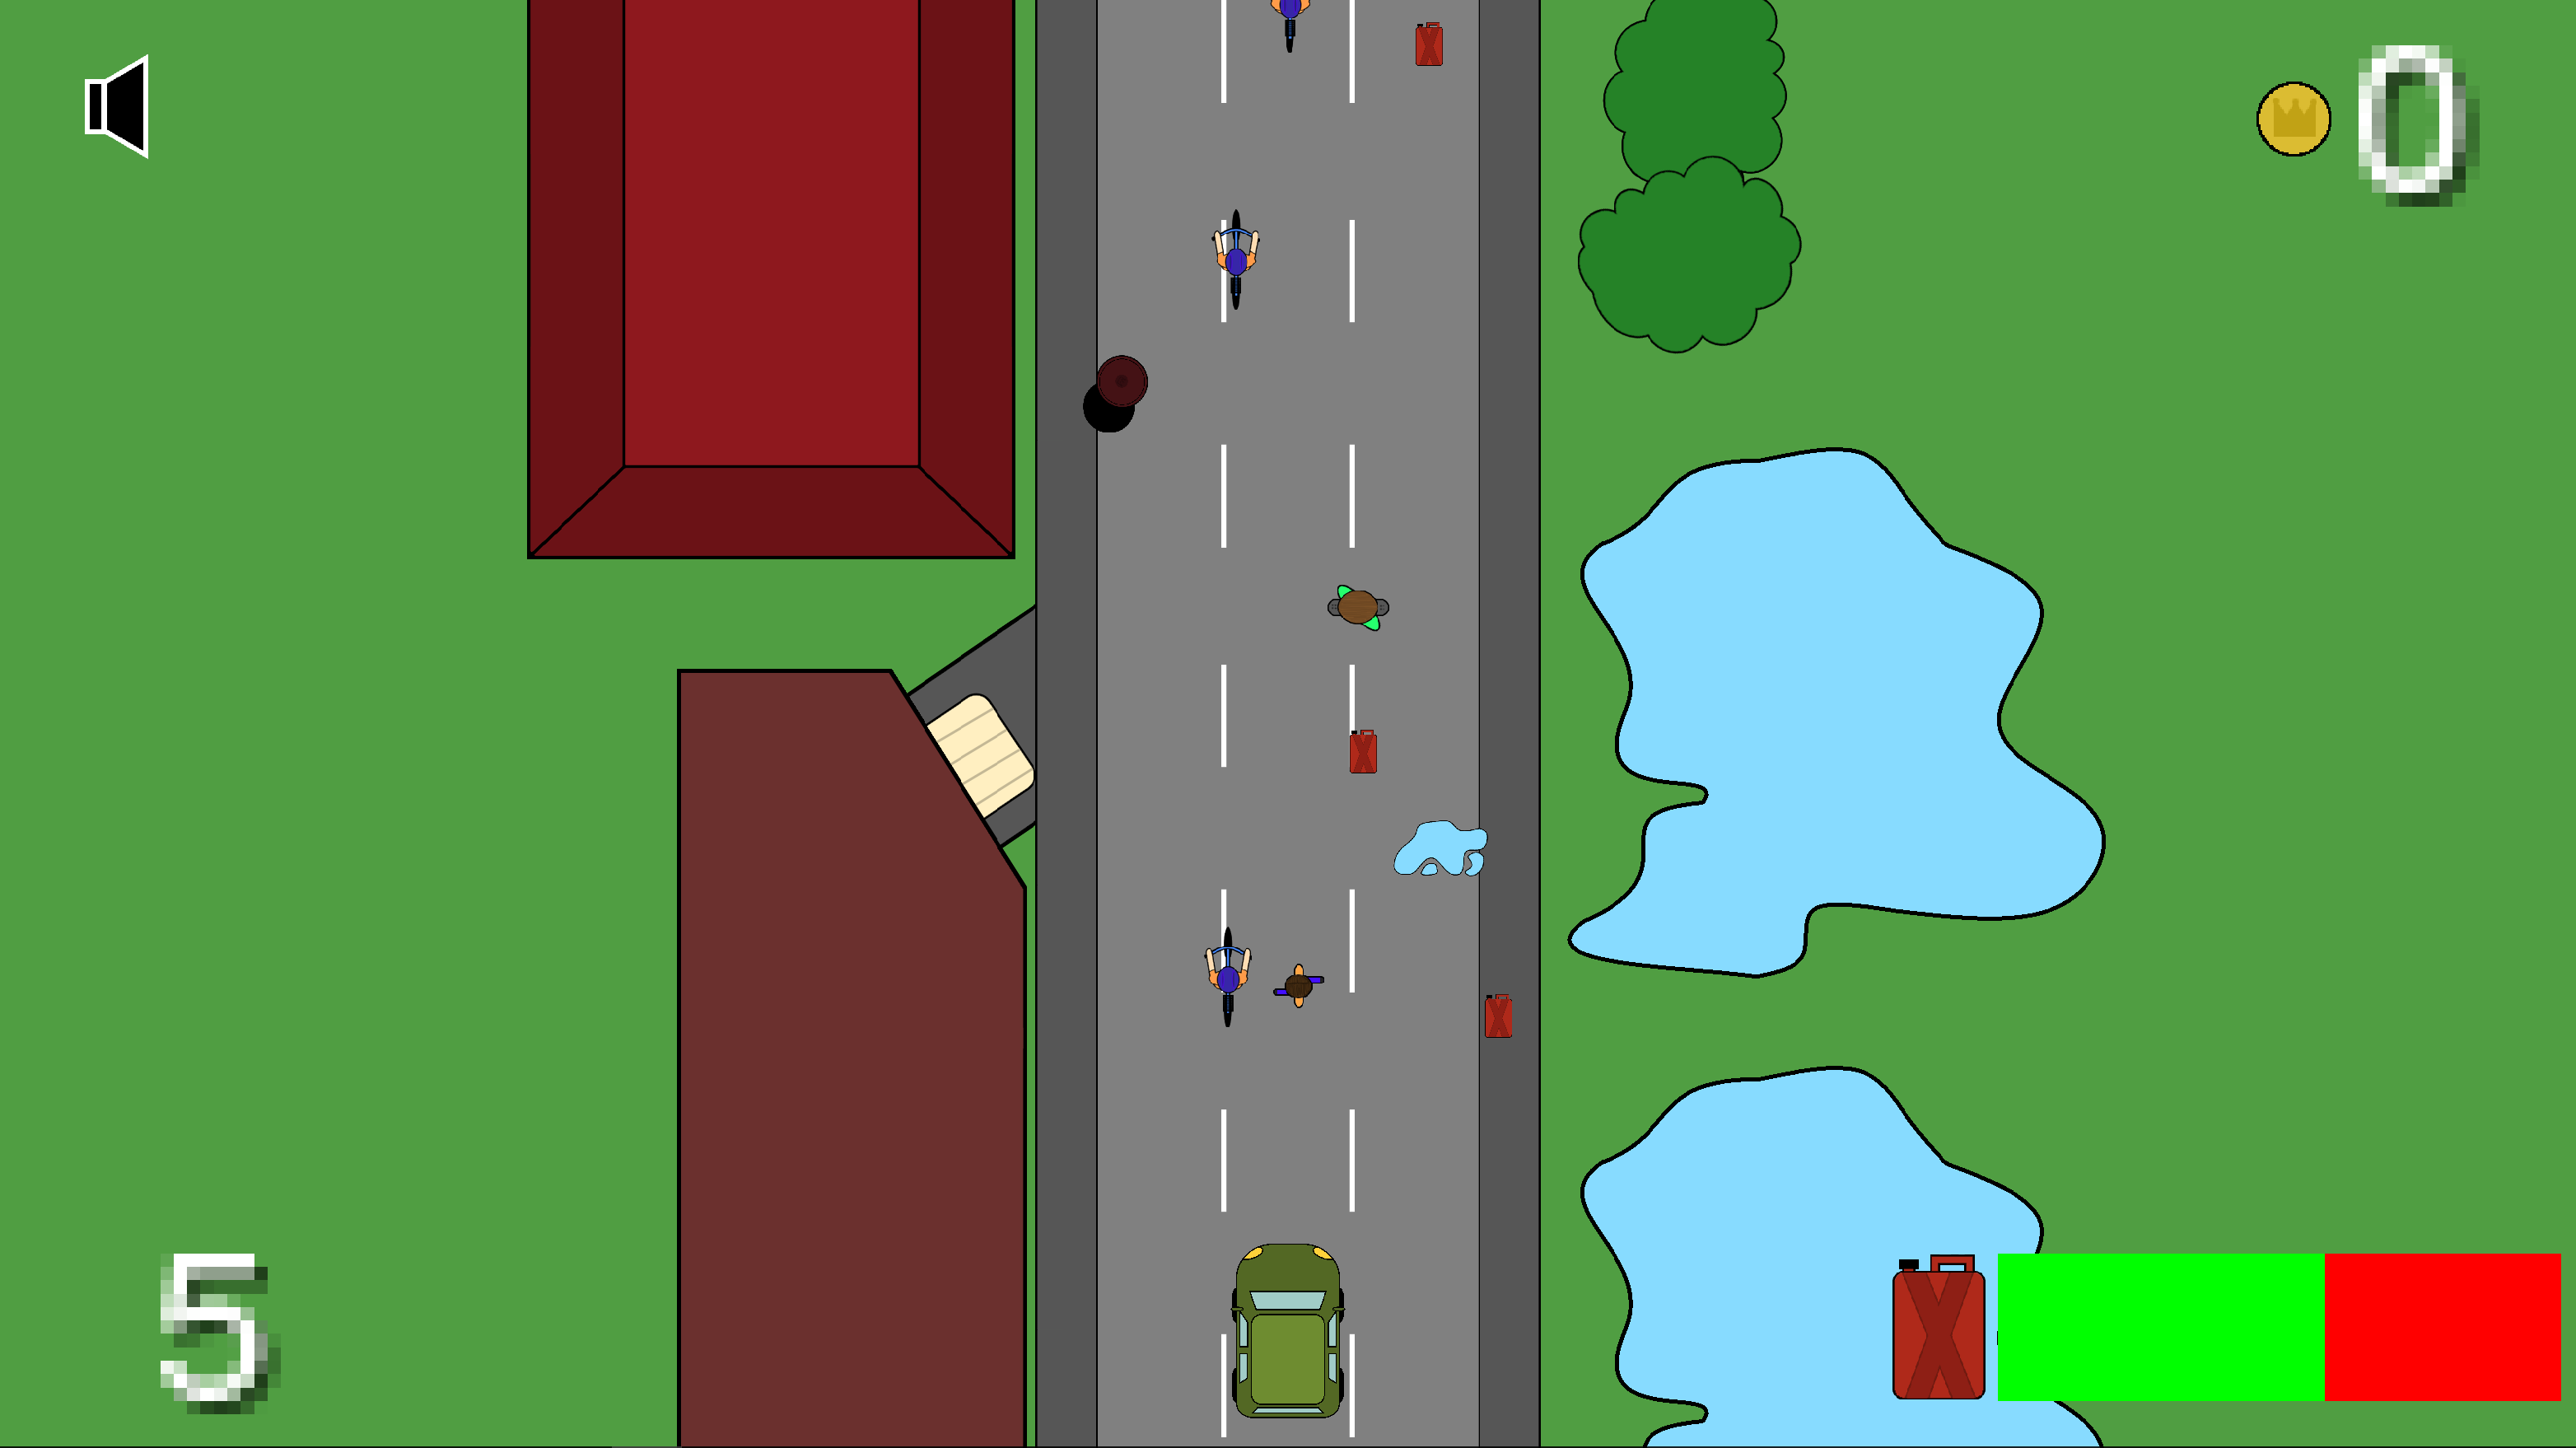
\includegraphics[width=1.00\textwidth]{images/game.PNG}}}
			\item {\hfil Figure 5. Gameplay}
			\bigskip
			\bigskip
			\bigskip
			\item{\makebox[13.5cm]{ 
\includegraphics[width=1.00\textwidth]{images/pause.PNG}}}
			\item {\hfil Figure 6. Pausemeny}
			\bigskip
			\bigskip
			\bigskip
			\item{\makebox[13.5cm]{ 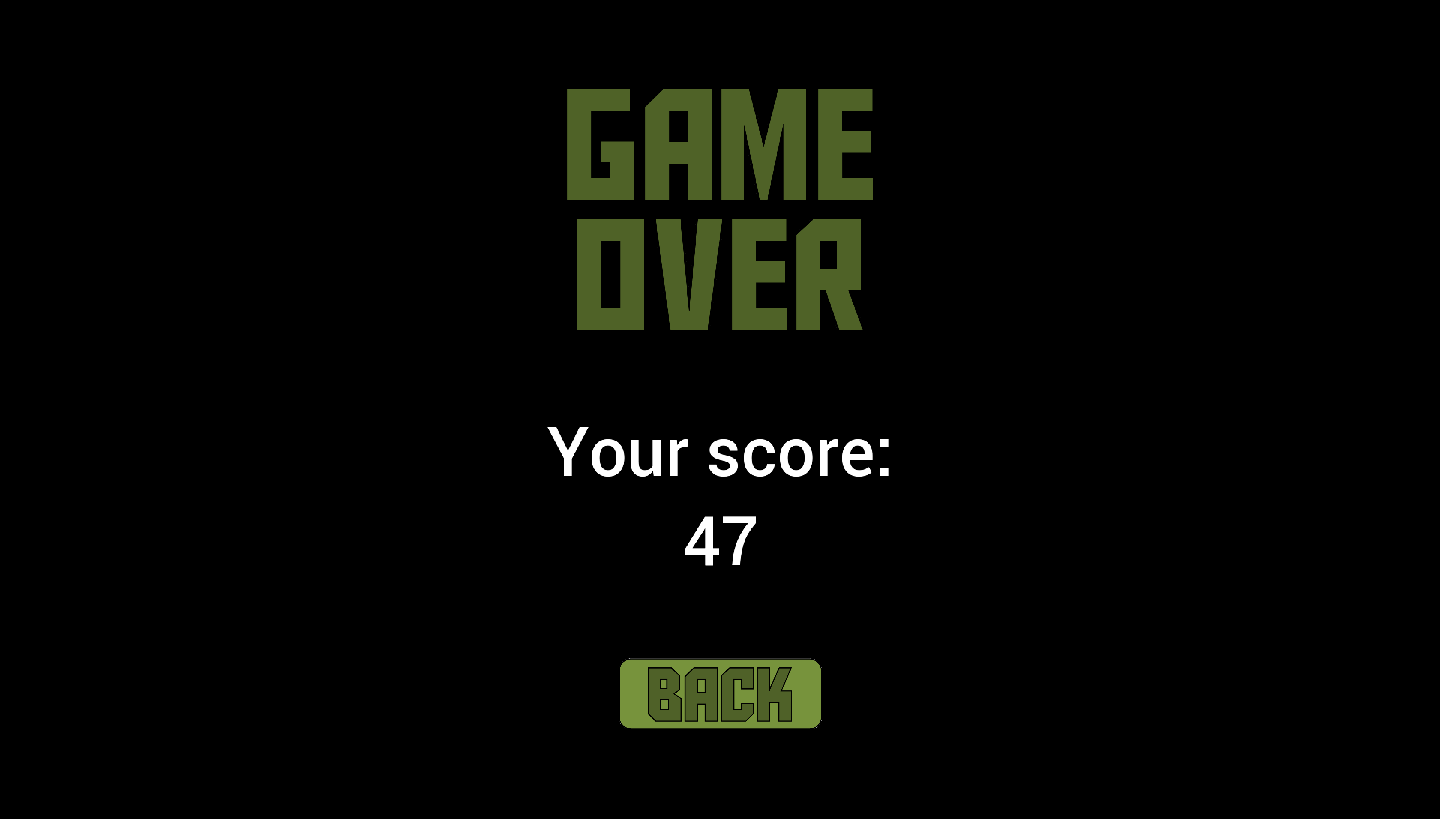
\includegraphics[width=1.00\textwidth]{images/gameover.PNG}}}
			\item {\hfil Figure 7. Game-over}
		\end{itemize}
	}
	\end{center} 

\newpage
\section{Credits}
\begin{center} 
\textbf{TeamDank}\\ \

\textbf{Utvikler team:}\\
TeamDank Programming Team\\ \

\textbf{Grafikk:} \\
TeamDank Art Department \\ \


\textbf{Værdata:} \\ 
Weather forecast from Yr, delivered by the Norwegian Meteorological Institute and NRK. \\ 
http://om.yr.no/verdata/xml/  \\
(Data from http://www.yr.no/sted/Hordaland/Bergen/Bergen/) \\ \

\textbf{Lyder:} \\ 
Lyder brukt fra freesound: \\
car\textunderscore drive.wav (In Car Driving.aif) by (http://freesound.org/people/RutgerMuller/) \\
happy\textunderscore bgmusic.wav (Happy 8bit Loop 01) by (http://freesound.org/people/Tristan\textunderscore Lohengr) \\
car\textunderscore crash.mp3 (Car Crash) by (http://freesound.org/people/squareal) \\
coin\textunderscore sound.wav (Coins 1) by (http://freesound.org/people/ProjectsU012) \\
dead\textunderscore pedestrian (me\textunderscore ouch.wav) by (http://freesound.org/people/SpazTastic) \\
fuel.wav (Drip2.wav) by (http://freesound.org/people/Neotone) \\
splash.mp3 (Splash 1.wav) by (http://freesound.org/people/FreqMan) \\ \

\textbf{Utviklere}: \\
Peter Andre Johansen \\
Håvar Eggereide \\
Kenneth Apeland \\
Philip Thao Hoang \\
Markus Johan Ragnhildstveit \\
Torbjørn Ola Sunnarvik Moen \\
Elias Refvem Siljan \\
Sturle Fraga Elvestad \\
Eirik Strøm \\
Amund Lindberg \\
Ole Magnus Lie \\
Bjørnar Herland \\ \

\textbf{Grafikk:} \\
Malin Øien \\
Emilia Botnen Van den Bergh \\ \

\textbf{Coach:} \\
Gunnar Schulze \\ \ 

\textbf{Juridisk Team:} \\ 
Anna Fossen-Helle \\ \

\textbf{Spillidé:} \\
Team 1\textunderscore9 \\
Kenneth Apeland \\
Natalie Priyaphon Wannaphong \\
Joakim Moss Grutle \\
Peder Ben \\ \
\end{center}

\end{document}